\documentclass[aps, 12pt]{revtex4}
\usepackage[english]{babel}
\usepackage[utf8]{inputenc}
\usepackage[T1]{fontenc}
% \usepackage{NotesTeX}
\usepackage{subfigure}
\usepackage{tikz}
\usetikzlibrary{arrows}
\usepackage{multirow}
\usepackage{listings}
\usepackage{extarrows}
\usepackage{parskip}
\usepackage{eurosym}
\usepackage{footmisc}
\usepackage{kantlipsum}
\usepackage{algorithm}
\usepackage{algpseudocode}


\def\thesection{\arabic{section}}
\def\thesubsection{\arabic{subsection}}
% \def\thesection{\arabic{section}}
\setcounter{secnumdepth}{4}


\renewcommand{\deg}{^{\circ}}
\newcommand\numberthis{\addtocounter{equation}{1}\tag{\theequation}}
\newcommand{\hksqrt}[2][]{\ \mathpalette\DHLhksqrt{[#1]{#2\,}}}
\def\DHLhksqrt#1#2{\setbox0=\hbox{$#1\sqrt#2$}\dimen0=\ht0
    \advance\dimen0-0.3\ht0
    \setbox2=\hbox{\vrule height\ht0 depth -\dimen0}
    {\box0\lower0.65pt\box2}}

\graphicspath{{figs/}}
\newcommand{\includegraphicsmaybe}[2][]{\IfFileExists{../plots/#2}{\includegraphics[#1]{#2}}{\includegraphics[width=0.75\linewidth]{giffel.jpg}}}



\begin{document}

\author{Håkon Olav Torvik}
\title{\Huge Problem Set 7 \\ \small Math228B Numerical solutions to differential equations}
\affiliation{UC Berkeley}
\date{\today}


\maketitle

\section*{Discontinuous Galerkin Method}
\subsection*{Convection}
I improve upon the \texttt{dgconvect0} in the ways specified. I elaborate more on the technical details of this on the code. To show that the plotting is better I include a figure of the solution at $t=T$ for the convection, using $n=6$ and $p=2$, in figure \ref{fig_convect_final_u}. As is excpected, with such low number of elements and polynomial degree, the solution does not very closely follow the exact solution, and decreases in magnitude as it moves to the right.


\begin{figure}
    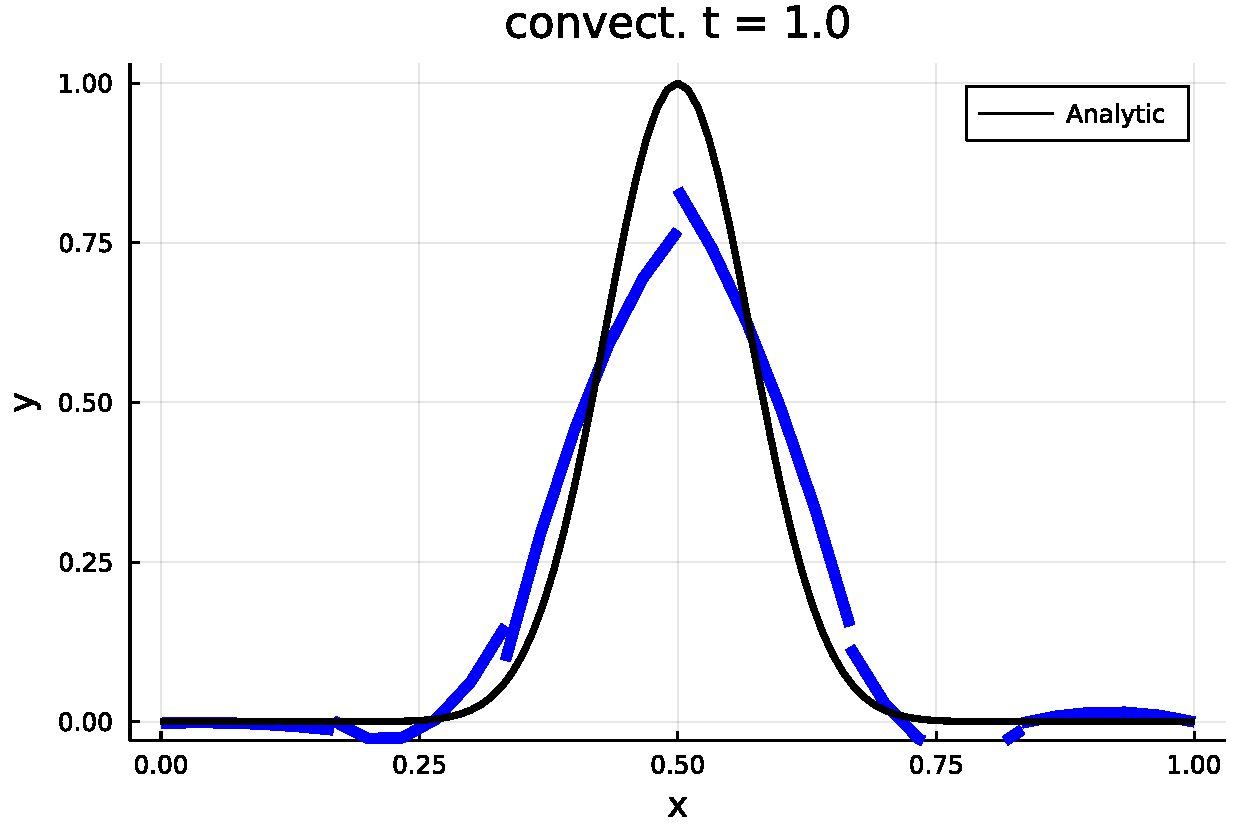
\includegraphics[width=0.75\linewidth]{u_finalconvect.pdf}
    \caption{Solution at $t=1$, using $n=6$, and $p=2$. It is clear that the plotted solution is a 2nd degree polynomial at each of the elements.}
    \label{fig_convect_final_u}
\end{figure}

The errors found with the convergence test are shown in figure \ref{fig_convect_errors}. The behaviour is as expected, with the error going down for higher polynomial degree and number of elements. Using logarithmic regression, I find that $\text{slope} = 3.2\log{(p)}$ gives a good model for the slopes. However, the theory gives that the error should go as $\mathcal{O}(h^{p+1})$.

\begin{figure}
    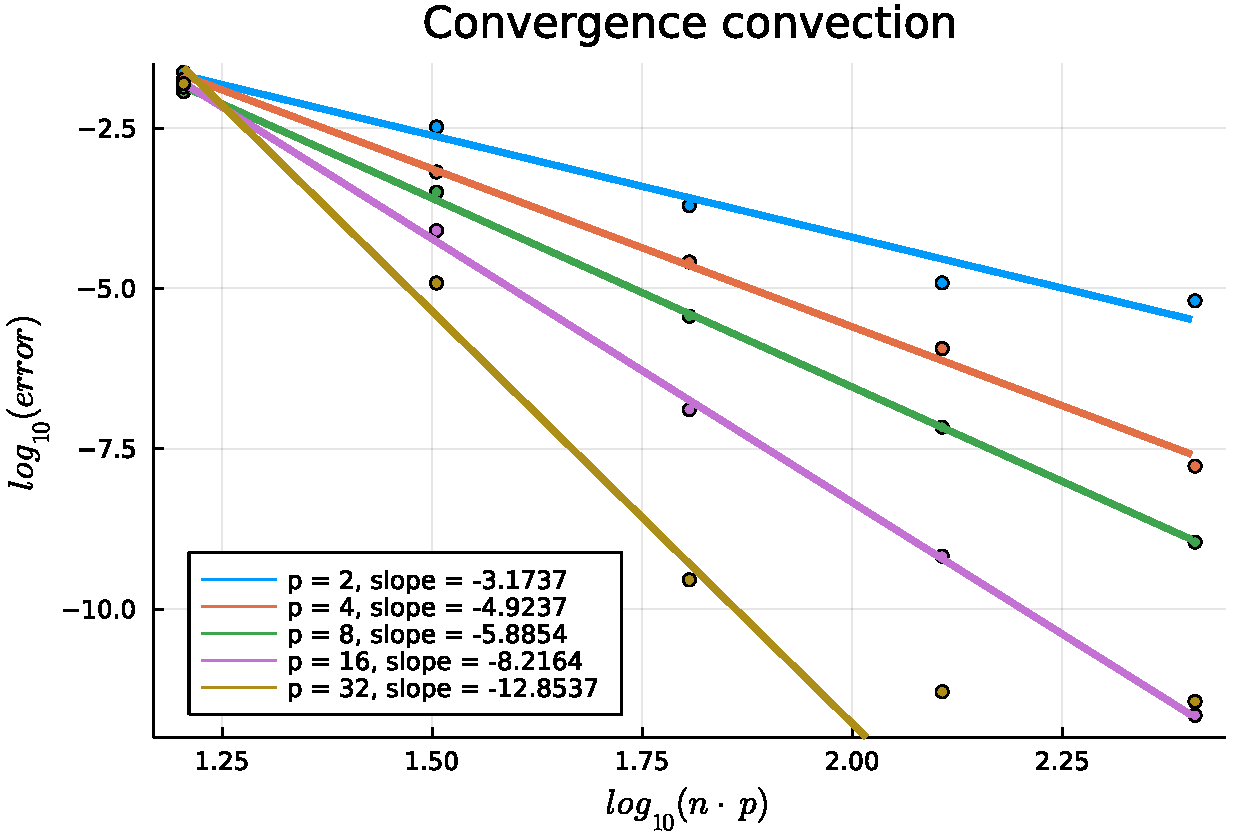
\includegraphics[width=0.75\linewidth]{conv_conv.pdf}
    \caption{Error convergence for the convection problem. The error goes down as number of elements and polynomial degree goes up. For the highest polynomial degree, the errors hit numerical presicion for the two largest number of elements. These points are not included in the slope-estimation. }
    \label{fig_convect_errors}
\end{figure}

\subsection*{Convection-diffusion}
To add diffusion to the problem, I change the function that calcualates the right-hand side of the differential equation, using the LDG method from the slides. Otherwise, the code is exactly similar.

As before, I plot the final solution with $n=6$ and $p=2$. This is shown in figure \ref{fig_convdiff_final_u}. Now the exact solution also decreases in magnitude, so the numerical solution isn't as bad for these parameters. The errors and slopes obtained from the same convergence test as before are shown in figure \ref{fig_convdiff_errors}. This is very similar to the convection plot, but some slopes are a little diferent, most notable the one for $p=32$. In  order to obtain the error for $p=32$ and $n\cdot p=256$, I had to use $dt=10^{-5}$, otherwise, the solution would explode.

\begin{figure}
    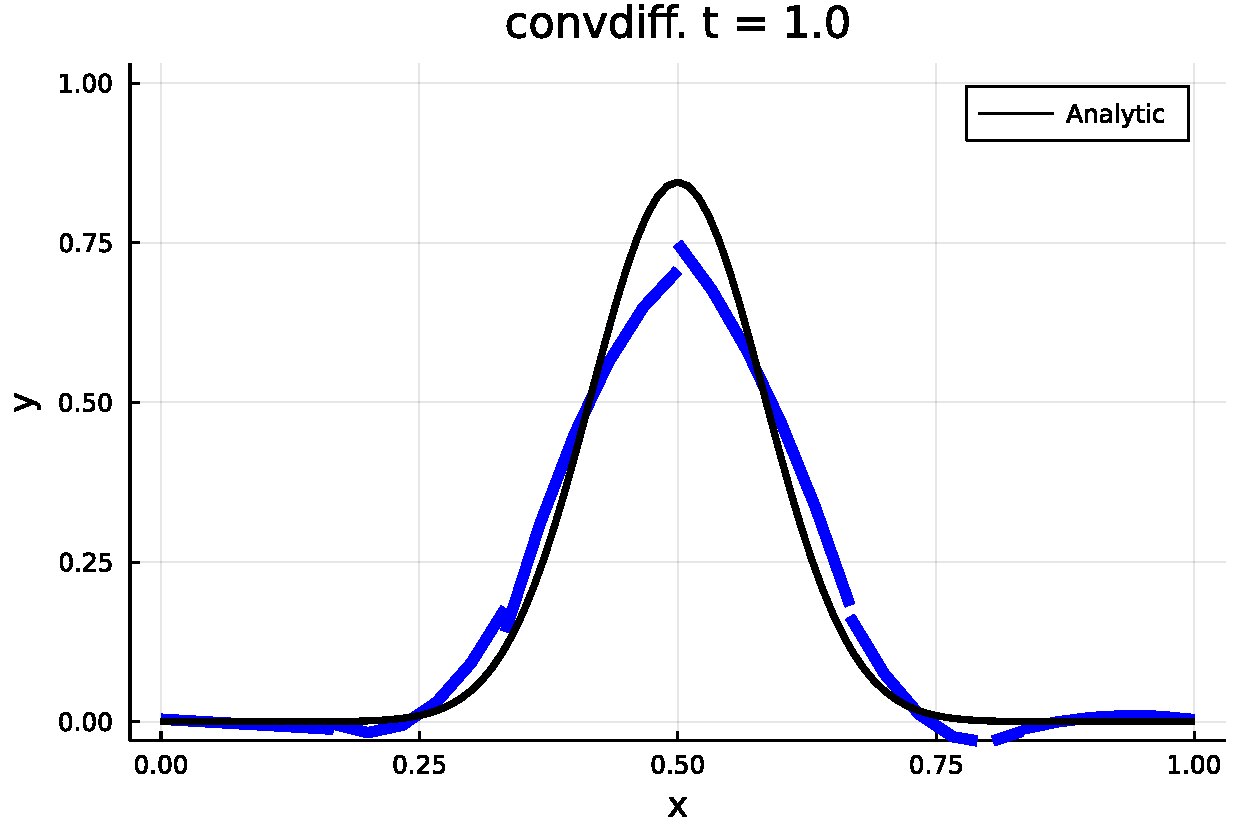
\includegraphics[width=0.75\linewidth]{u_finalconvdiff.pdf}
    \caption{Solution at $t=1$, using $n=6$, and $p=2$.}
    \label{fig_convdiff_final_u}
\end{figure}

\begin{figure}
    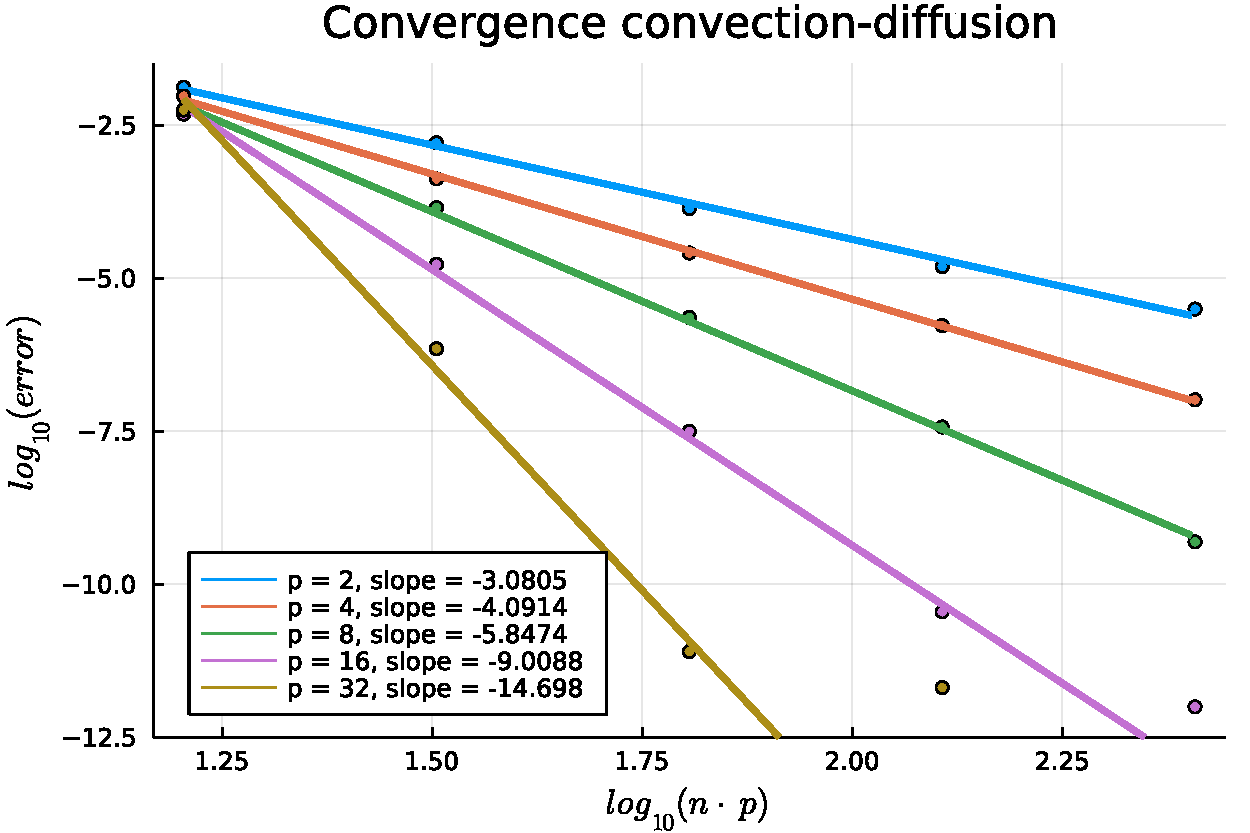
\includegraphics[width=0.75\linewidth]{conv_diff.pdf}
    \caption{Error convergence for convection-diffusion problem. }
    \label{fig_convdiff_errors}
\end{figure}


\end{document}

